\documentclass[../../main.tex]{subfiles}


\begin{document}
\subsection*{(a)}
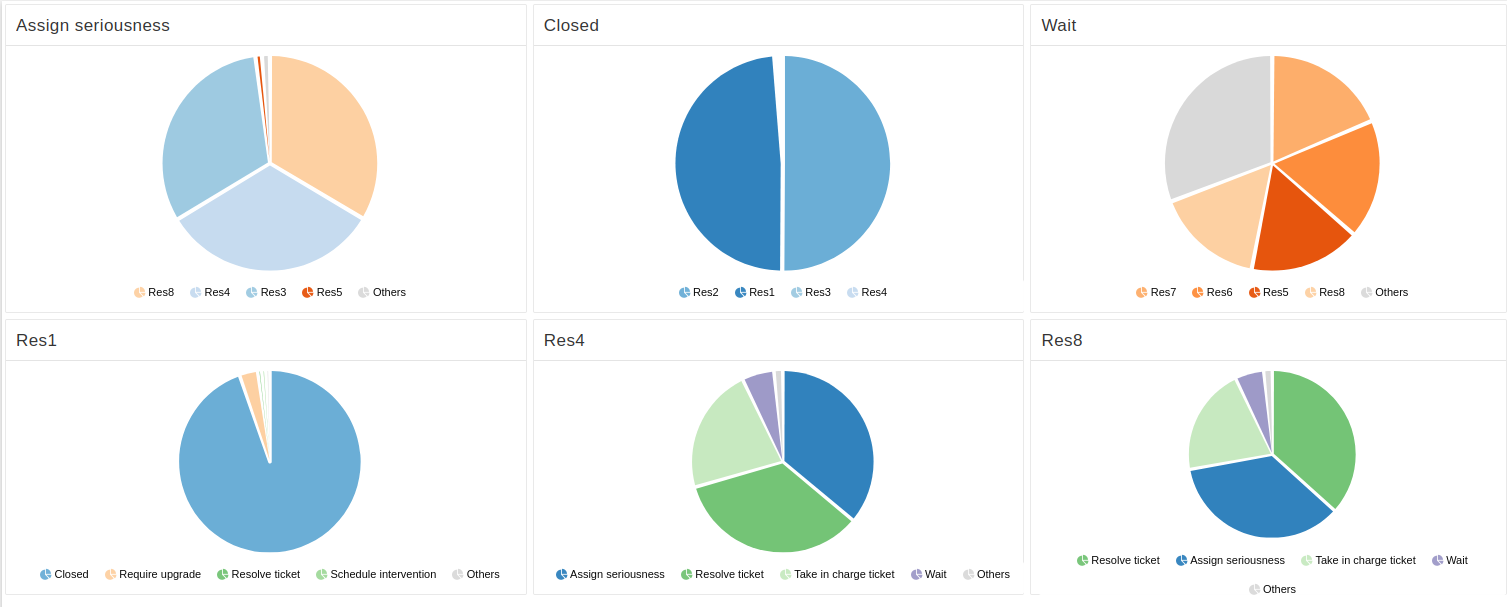
\includegraphics[width=\columnwidth]{img/Celonis_a_Visualization.png}\\
For the left Pie Chart we used \verb|"event_table_csv"."RESOURCE"| as the Dimension and \verb|COUNT("event_table_csv"."ACTIVITY")| as the KPI.\\
For the right Pie Chart we used \verb|"event_table_csv"."ACTIVITY"| as the Dimension and \verb|COUNT("event_table_csv"."RESOURCE")| as the KPI.


\subsection*{(b)}
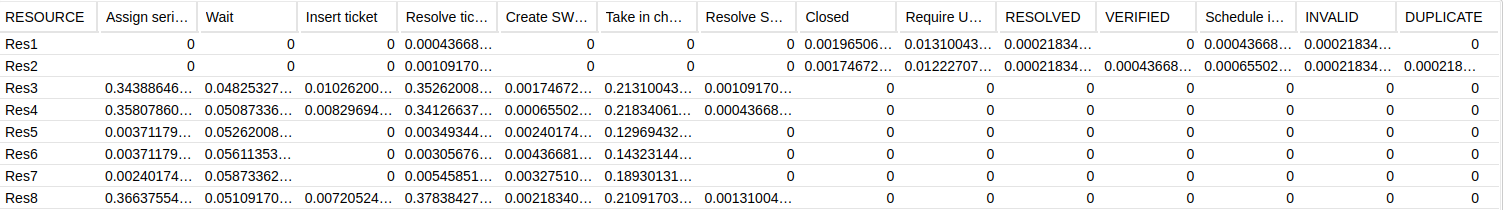
\includegraphics[width=\columnwidth]{img/Celonis_b_OLAP.png}\\
\begin{verbatim}
	SOURCE("event_table_csv"."RESOURCE")
\end{verbatim}
\begin{lstlisting}
	SUM(CASE WHEN SOURCE ( "event_table_csv"."ACTIVITY" ) = '[ACTIVITY]' THEN 1 ELSE 0 END) / 4580
\end{lstlisting}
Replace \verb|[ACTIVITY]| with each of the 14 Activities for the corresponding Dimensions. 4580 is the number of cases obtained by \verb|COUNT_TABLE("case_table_csv")|.

\subsection*{(c)}

\subsection*{(d)}
\includegraphics[width=\columnwidth]{img/Celonis_d_OLAP.png}\\
\begin{verbatim}
	SOURCE("event_table_csv"."RESOURCE")
\end{verbatim}
\begin{verbatim}
	TARGET("event_table_csv"."RESOURCE")
\end{verbatim}
\begin{lstlisting}
	COUNT(SOURCE("event_table_csv"."ACTIVITY")) / 4580
\end{lstlisting}
4580 is the number of cases obtained by \verb|COUNT_TABLE("case_table_csv")|.

\subsection*{(e)}

\subsection*{(f)}

\subsection*{(g)}

\end{document}